% !TEX root =  ../Dissertation.tex

\chapter{Project Management}

The project timeline is shown in the Gantt chart (\cref{fig:Gantt}). During the
first two months, the focus was on developing Agda Tree and Agda Comp. For Agda
Tree, the initial milestone was parsing an Agda project to extract the
definition dependency graph. The next step involved implementing queries for
this graph. Once the queries were functional, the final milestone was creating
the CLI that allowed users to execute these queries. The queries were then
unit tested for correctness and performance and a stable version of
the CLI tools was finished by the demonstration date.

At the same, Agda Comp was being developed. The first task was exploring
various compilation strategies and methods to compile an Agda project. After
selecting the strategies, they were tested for correctness, safety, and
compilation time, marking a major milestone. Following this, a CLI was
implemented to execute these strategies, and this was also completed by
the demonstration date.

An agile software development methodology was used throughout the project.
As shown in the timeline, multiple tasks ran concurrently until they were
completed for the demonstration. Weekly meetings with my supervisor facilitated
iterative progress, where I presented a working state of the project along with
a summary of achievements since the previous meeting. My supervisor provided
feedback and suggestions for improvements or additions for the following week.
This iterative approach enabled rapid prototyping of tools that my supervisor
could test early in development.

\begin{figure}[H]
    \centering
    \label{fig:Gantt}
    \makebox[\textwidth]{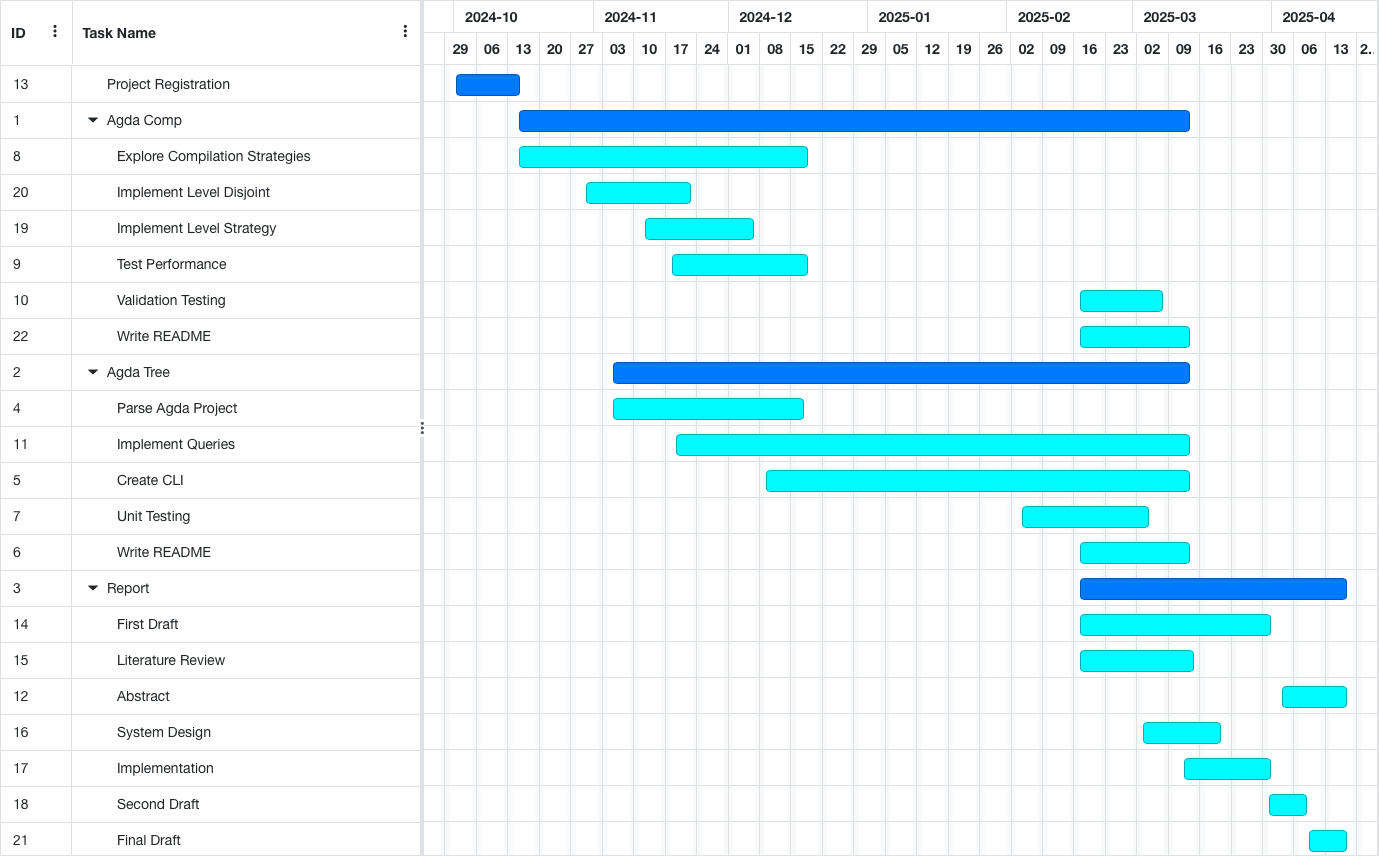
\includegraphics[width=\textwidth]{Gantt.png}}
    \caption{Gantt Chart}
\end{figure} 


% What is the timeline for your project? What software development
% methodology will you use? Can you identify the major milestones? These types of questions are
% important for project planning and should be addressed directly.
%
% \begin{itemize}
% \item Gantt chart 
% \item Weekly updates with supervisor 
% \item Getting the s-expression extractor was a major milestone 
% \item Using python instead of clojure was a significant improvement
% \end{itemize}
%
% | Week | Goal | Outcome |
% | ------------- | -------------- | -------------- |
% | S1.Wk1 <br> 30th September 2024  | Pick Project idea and analyze HTML files and explore what data can be accessed | Chose project idea, analysing agda HTML files for easier searching and created python script that reads Agda HTML files and returns all of the found symbols |
% | S1.Wk2 | Complete project registration and research related works | Registered project and learned about LSPs and Ctags but they don't quite match our use case. |
% | S1.Wk3 | Research and implement graphs |  |
% | S1.Wk4 | Implement some queries | |
% | S1.Wk5 | Implement some queries | |
% | S1.Wk6 | Implement some queries | |
% | S1.Wk7 | Implement some queries | |
% | S1.Wk8 | Implement some queries | |
% | S1.Wk9 | Implement some queries | |
% | S1.Wk10 |Test scalability | |
% | S1.Wk11 | Test scalability | |
% | CV1 | | |
% | CV2 | | |
% | CV3 | | |
% | CV4 | | |
% | S1.Wk12 | Write Introduction | |
% | S2.Wk1 | Write Literature review | |
% | S2.Wk2 | Write Legal/Social/Ethica issues | |
% | S2.Wk3 | Write requirements | |
% | S2.Wk4 | Write Design of the software | |
% | S2.Wk5 | Write how I implemented the software | |
% | S2.Wk6 | Write testing and success Measurement | |
% | S2.Wk7 | Write Project Management | |
% | S2.Wk8 | Write Evaluation | |
% | S2.Wk9 | Proof read | |
% | S2.Wk10 | Proof read | |
% | S2.Wk11 | Write abstract | |
% | EV1 | Proof read | |
% | EV2<br>  5pm on 17th April 2025 | | |
